\documentclass[12pt]{article}
% Эта строка — комментарий, она не будет показана в выходном файле
\usepackage{ucs}
\usepackage[utf8x]{inputenc} % Включаем поддержку UTF8
\usepackage[russian]{babel}  % Включаем пакет для поддержки русского языка
\usepackage{amsmath}
\usepackage{mathtools}
\usepackage{amssymb}
% \usepackage[dvips]{graphicx}
% \graphicspath{{noiseimages/}}
\usepackage[pdftex]{graphicx}


% Параметры страницы: 1см от правого края и 2см от остальных.


\hoffset=0mm
\voffset=0mm
\textwidth=180mm        % ширина текста
\oddsidemargin=-6.5mm   % левое поле 25.4 - 5.4 = 20 мм
\textheight=240mm       % высота текста 297 (A4) - 40
\topmargin=-15.4mm      % верхнее поле (10мм)
\headheight=5mm      % место для колонтитула
\headsep=5mm          % отступ после колонтитула
\footskip=8mm         % отступ до нижнего колонтитула


\begin{document}
    \author {Зотов Алексей 496 гр.}
    \title {Лабораторная работа 1.3 \\  Изучение колебаний на примере физического маятника}
    \maketitle{}   

    \indent
    \textbf{Цель работы:} исследовать физический и математический маятники
    как колебательные системы, измерить зависимость периода колебаний физического маятника от его момента инерции.
    \\ \\
    \indent
    \textbf{В работе используются:} физический маятник (однородный стальной стержень), опорная призма, математический маятник, счётчик числа колебаний, линейка, секундомер.

    \begin{center} 
        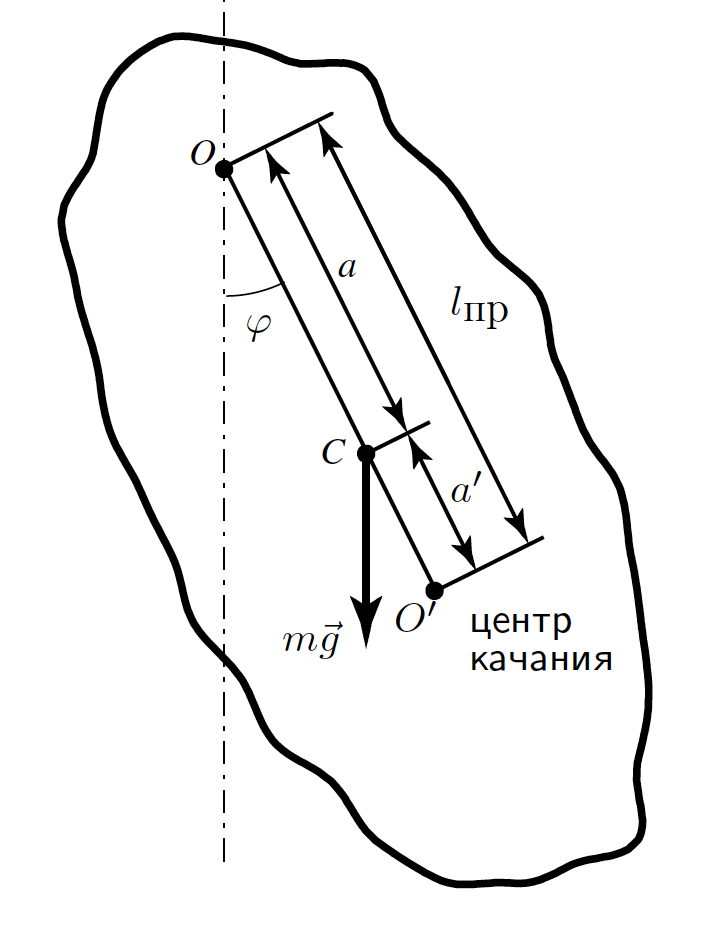
\includegraphics[width=1.5in]{phys_mtn.png} \\ Рис. 1: физический маятник.
    \end{center}
    
    % ДОБАВИТЬ ТЕОРИЮ

    \textbf{Экспериментальная установка.}
    В данной работе в качестве физического маятника используется однородный стальной стержень длиной
    $l$  На стержне закрепляется опорная призма, острое ребро
    которой является осью качания маятника. Призму можно перемещать
    вдоль стержня, меняя расстояние $a$ от точки опоры (точки подвеса)
    маятника до его центра масс. Используя теорему Гюйгенса–Штейнера 
    и считая стержень тонким (его радиус много
    меньше длины), вычислим его момент инерции:
    \begin{equation}
        I = \frac{ml^2}{12} + ma^2
    \end{equation}

    \textbf{Ход работы}
    \begin{enumerate} 
        \item Проведем $n = 6$ экспериментов, в каждом измерим время $N_T = 20$ полных колебаний маятников.
        \begin{enumerate}
            \item \underline{Физический маятник.}
            \begin{table}[h]
                    \caption{Время 20 полных колебаний}
                    \begin{center}
                    \begin{tabular}{|c|c|c|c|c|c|c|}
                            \hline 
                                $i$ & 1 & 2 & 3 & 4 & 5 & 6 \\
                            \hline
                                $t_{20} , (c)$ &31.43&31.72&31.56&31.62&31.49&31.53\\
                            \hline
                            \end{tabular}
                        \end{center}
            \end{table}

            Среднее значение $t_{avg} = 31.56$. Среднее значение периода $T_{avg} = t_{avg}/20 = 1.5779$[c].
            Среднеквадратичное отклонение измерения:
            $\sigma = \sqrt{\frac{\Sigma (t_i - t_{avg})^2 }{n-1}} \approx 0.10187$ \\
            Относительная погрешность периода: $\varepsilon = \frac{\sigma}{N* T_{avg}} \approx 0.0032 < 0.005$ \\  
        \item \underline{Математический маятник.}
            \begin{table}[h]
                    \caption{Время 20 полных колебаний}
                    \begin{center}
                    \begin{tabular}{|c|c|c|c|c|c|c|}
                            \hline 
                                $i$ & 1 & 2 & 3 & 4 & 5 & 6 \\
                            \hline
                                $t_{20} , (c)$ &31.56&31.34&31.6&31.62&31.63&31.54\\
                            \hline
                            \end{tabular}
                        \end{center}
            \end{table}

            Среднее значение $t_{avg} = 31.548$. Среднее значение периода $T_{avg} = t_{avg}/20 = 1.5774$[c].
            Среднеквадратичное отклонение измерения:
            $\sigma = \sqrt{\frac{\Sigma (t_i - t_{avg})^2 }{n-1}} \approx 0.10780$ \\
            Относительная погрешность периода: $\varepsilon = \frac{\sigma}{N* T_{avg}} \approx 0.0034 < 0.005$ \\  
        \end{enumerate}
        \item Возбудим малые колебания физического маятника, отклонив на угол $A_0 = 10.0^o$. Измерим время $t$ затухания в $\approx 1.3$ раза по достижении маятником значения амплитуды $A_1 \approx 7.5^o$. \\
        $t \approx$ 5 мин 30 с = 330 (с). \\
        Количество колебаний $N = 209$.\\
        Добротность $Q = \frac{\pi}{\gamma_{e}T}$ , где $\gamma_{e} = 1 / \tau_{e}$ - величина обратная времени убавыния амплитуды $A$ в $e$ раз. Ее вычислим из закона убывания амплитуды: $\gamma_{e} = \gamma_{1.3} \ln{1.3}$, тогда :\\
        \begin{equation}
            Q = \frac{\pi \tau_{1.3}}{T \ln(1.3)} \approx 2504.23
        \end{equation}
        \item Найдем зависимость периода колебаний $T$ от расстояния $a$ между точкой опоры и центром масс.
        \begin{table}[h]
                    \caption{Время 20 полных колебаний}
                    \begin{center}
                    \begin{tabular}{|c|c|c|c|c|c|c|c|c|c|c|c|c|}
                            \hline 
                                $a,[cm]$ & 4.0& 8.0& 12.0& 16.0& 20.0& 24.0& 28.0& 32.0& 36.0& 40.0& 44.0& 48.0 \\

                            \hline
                                $t_{20},[c]$ & 53.87& 43.19& 36.68& 33.28& 31.69& 30.9& 30.57& 30.68& 31.13& 31.31& 31.85& 32.69 \\
                            \hline
                                $T,[c]$ & 2.693& 2.159& 1.834& 1.664& 1.585& 1.545& 1.528& 1.534& 1.556& 1.565& 1.593& 1.634\\
                            \hline
                            \end{tabular}
                        \end{center}
            \end{table}

        \begin{table}[h]
            \caption{Зависимость $[T^2 a ](a^2)$}
            \begin{center}
                \begin{tabular}{|c|c|c|c|c|c|c|c|c|c|c|c|c|}
                    \hline
                        $a^2 , [m^2]$ & 0.002 & 0.006 & 0.014 & 0.026 & 0.04 & 0.058 & 0.078 & 0.102 & 0.13 & 0.16 & 0.194 & 0.23 \\
                    \hline
                        $T^2 a , [c^2 m] $ & 0.29 & 0.373 & 0.404 & 0.443 & 0.502 & 0.573 & 0.654 & 0.753 & 0.872 & 0.98 & 1.116 & 1.282 \\
                    \hline
                \end{tabular}
            \end{center}
        \end{table}

        \begin{center} 
            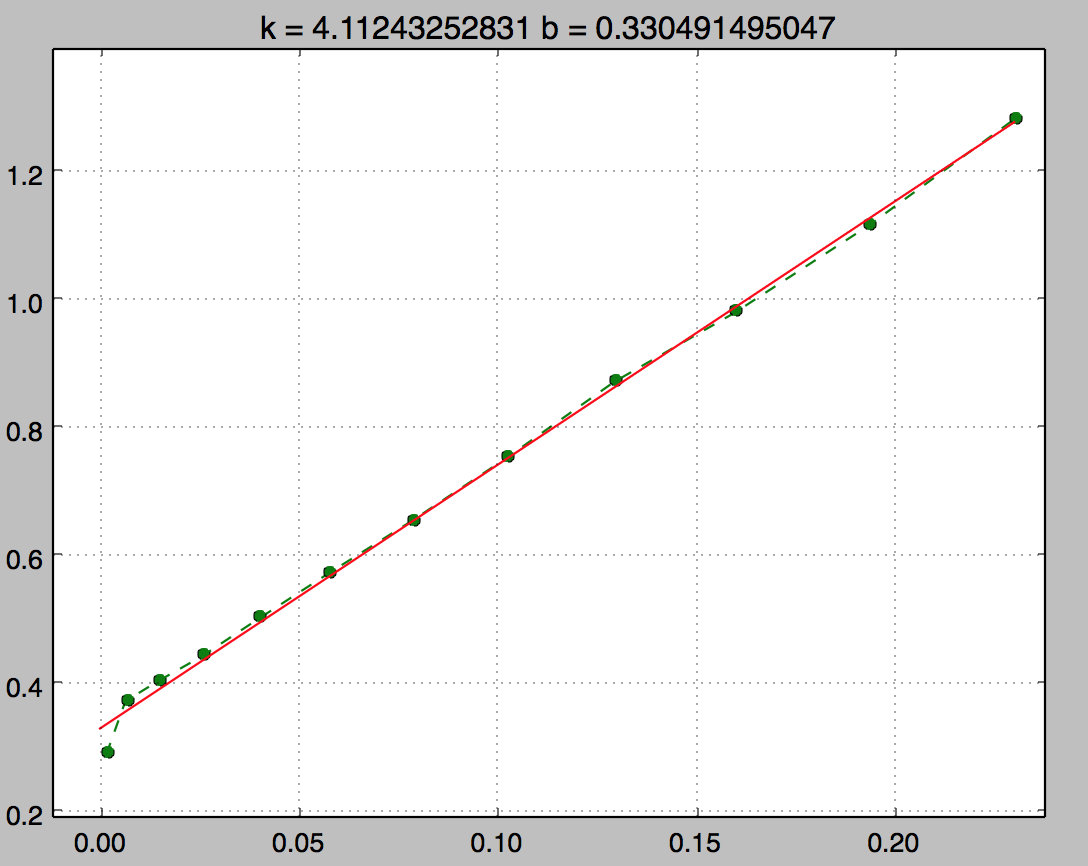
\includegraphics[width=5in]{figure.png} \\ Рис. 2: график $[T^2 a ] (a^2)$.
        \end{center}
        Аппроксимирующая по методу наименьших квадратов прямая $y = kx + b$ , где $k = 4.1124$, $b = 0.3305$.
        \\
        Используя формулу для рассчета момента инерции тонкого стержня:
        \begin{equation}
              T = 2 \pi \sqrt{\frac{a^2 + \frac{l^2}{12}}{ag}}     
        \end{equation}
        получим: 
        \begin{equation}
              T^2a = \frac{4 \pi^2 } {g} a^2 + \frac{\pi^2 l^2}{3 g}
        \end{equation}
        $\implies \frac{g}{4\pi^2} = \frac{1}{k} \approx 0.243 \implies g \approx 9.59 [\frac{m}{c^2}]$ \\
        $l = \sqrt{\frac{12b}{k}} \approx 0.982[m]$ \\
        % Рассчет погрешности: \\
        % \indent $\sigma_{k} \approx \frac{1}{\sqrt{n}} \sqrt{}$
        
    \end{enumerate} 
\end{document}
